\chapter{Time series problem with change point in test}
\label{app:timeseries-cpoint-problem} 

Unless it is specified otherwise, the miscoverage level was set to $\a=0.05$ (\textit{i.e.} $95\%$ of expected coverage) for the visualizations.

\begin{figure}[ht]
    \centering
    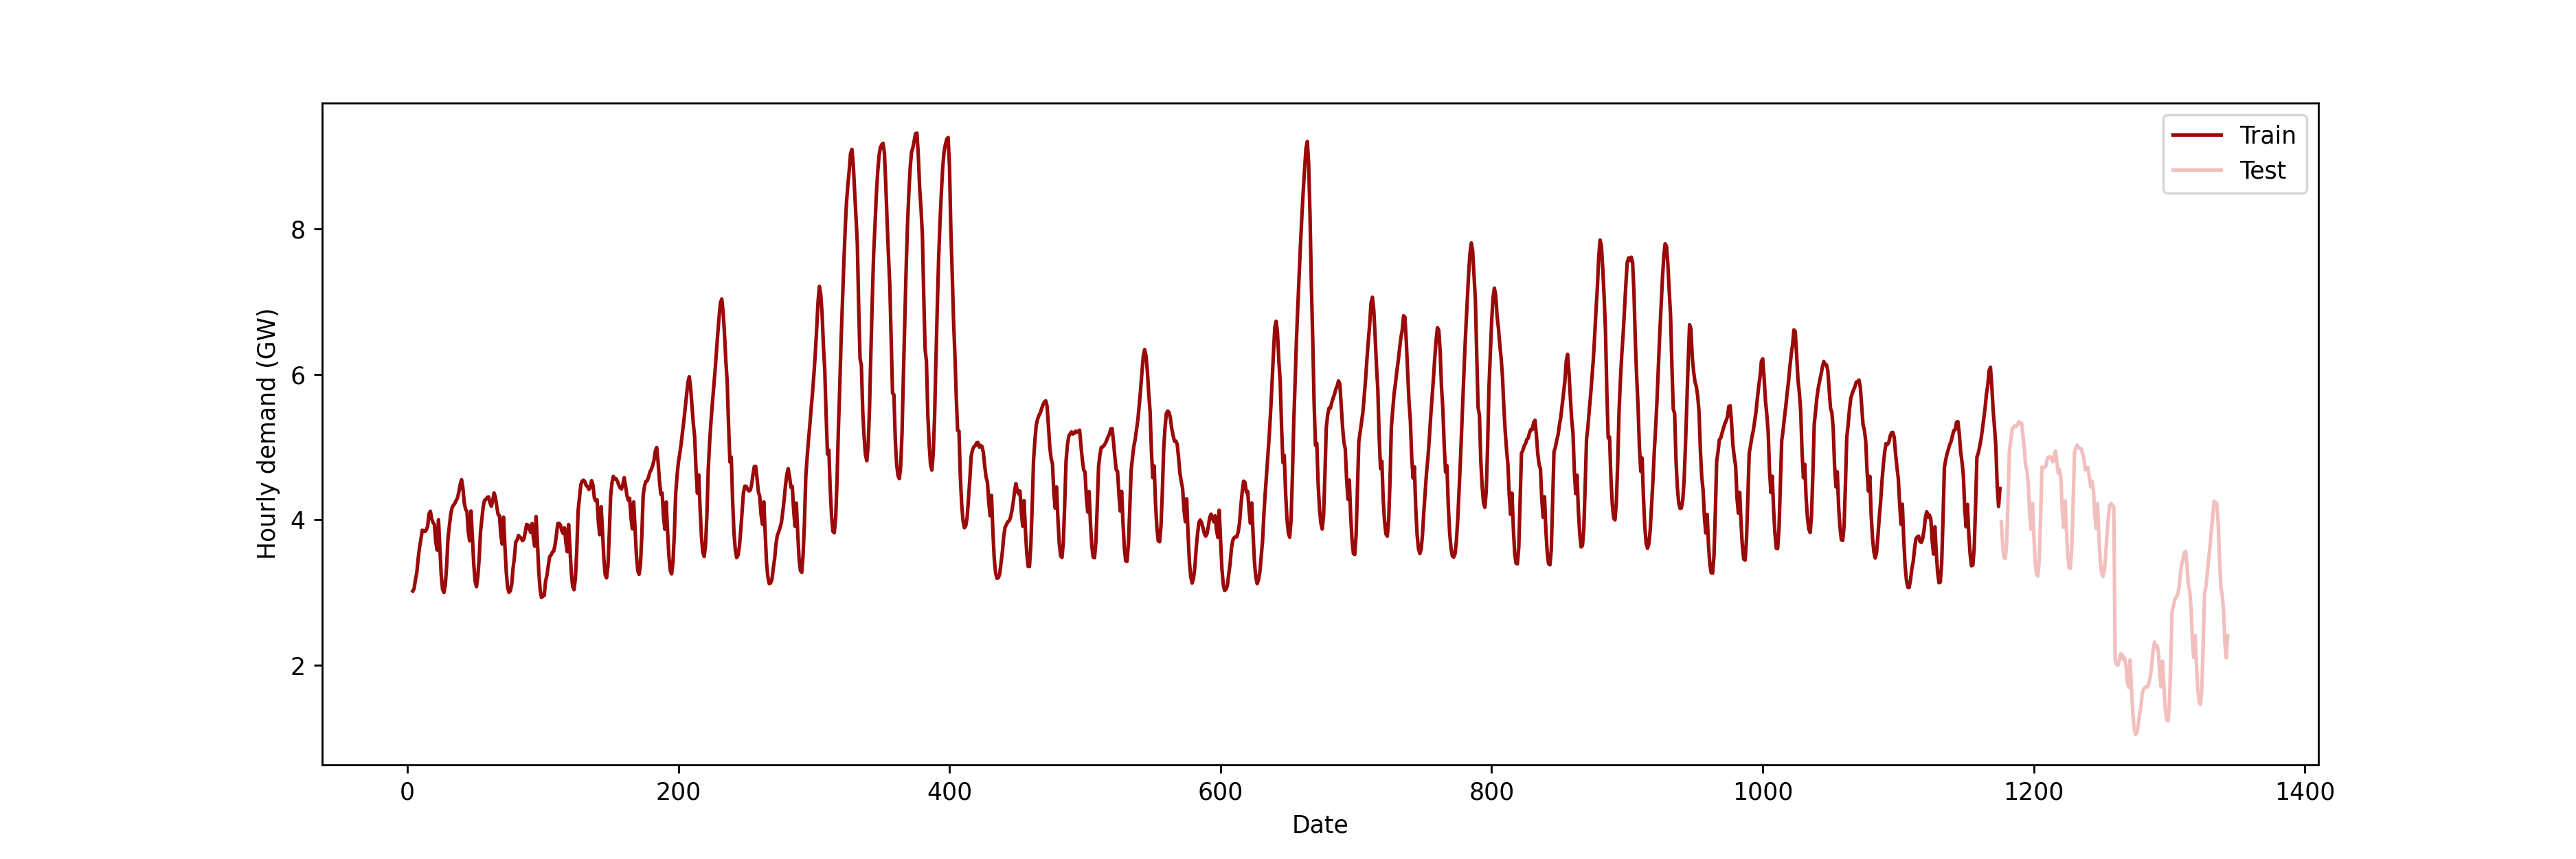
\includegraphics[width=1\textwidth]{Figures/timeseries/with-change-point/data-with-change-point-timeseries.png}
    \caption{Time series problem's dataset when a change point is added to the test split.}
    \label{fig:app-timeseries-data-cpoint}
\end{figure}

\begin{figure}[ht]
    \centering
    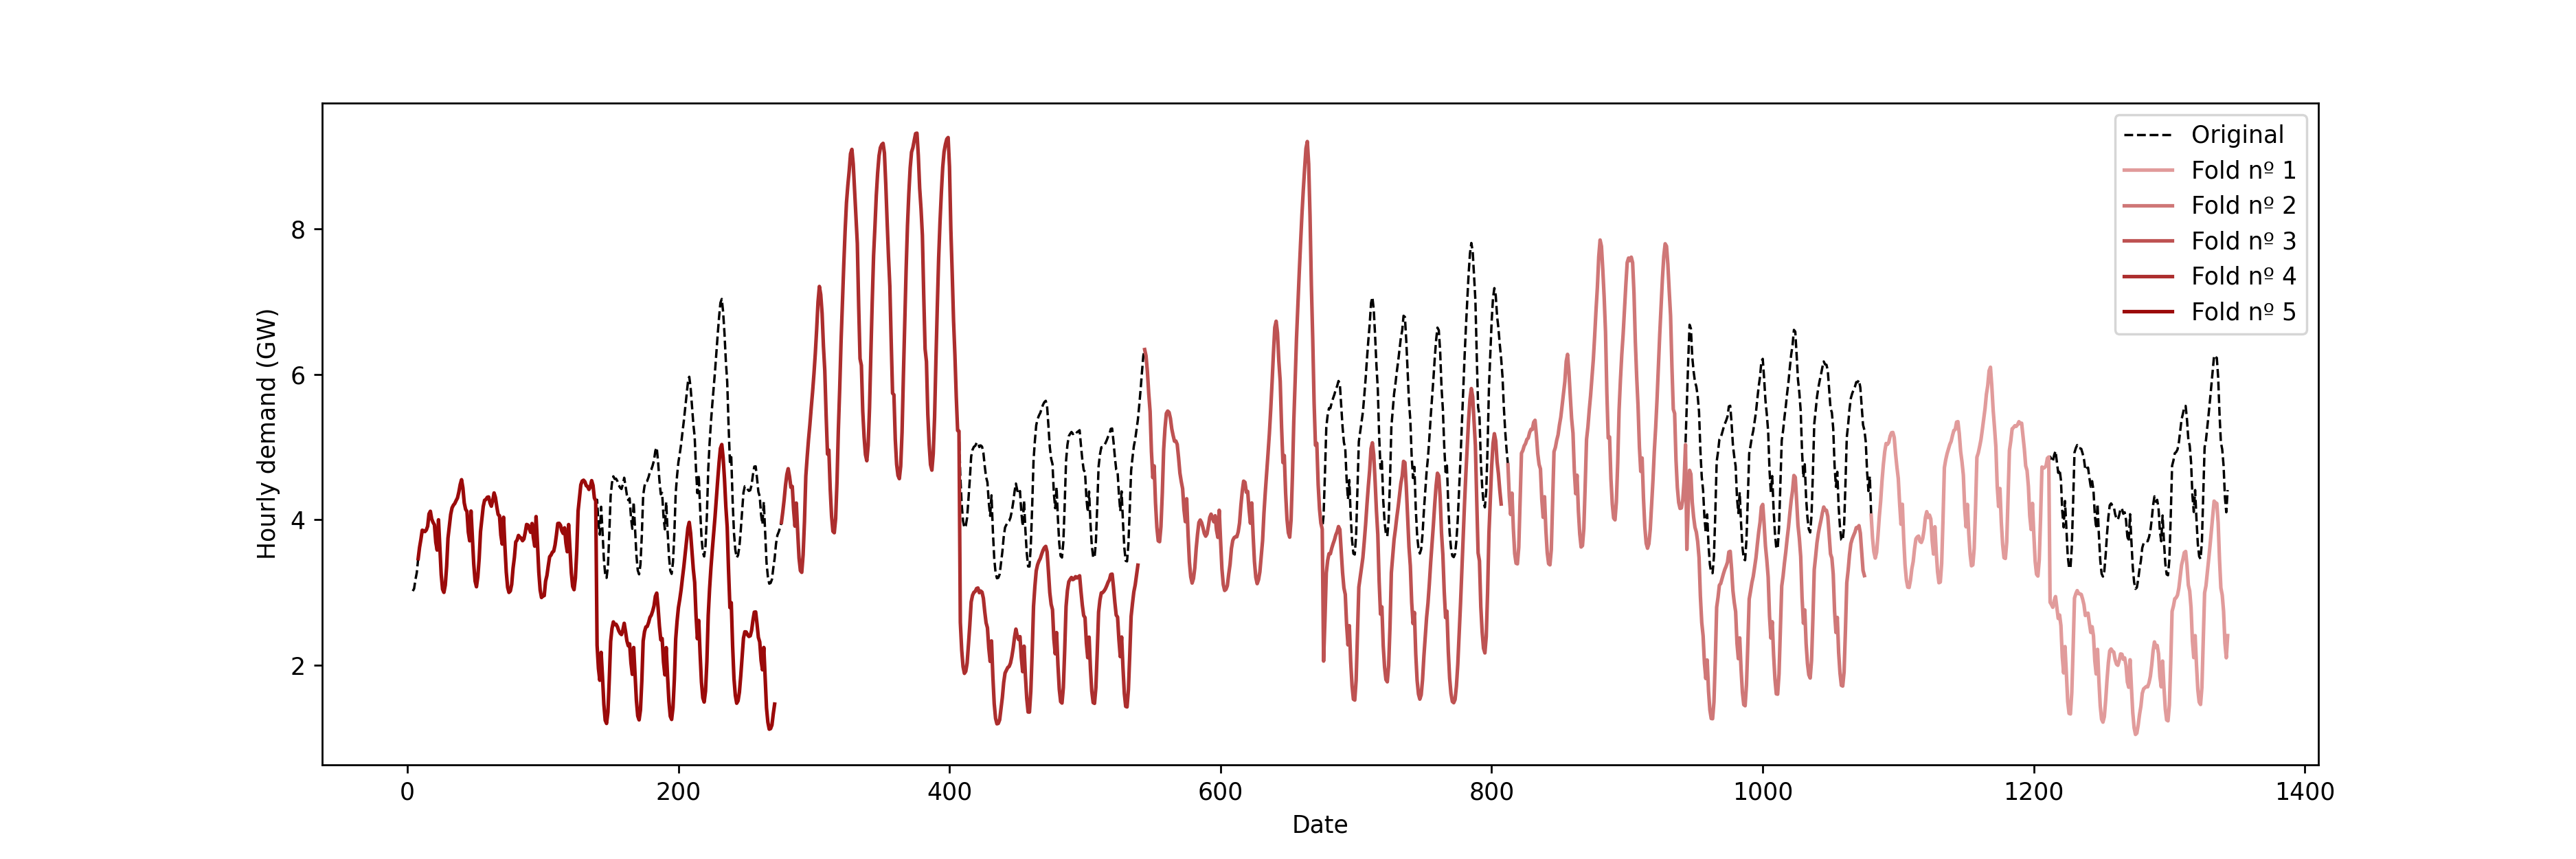
\includegraphics[width=1\textwidth]{Figures/timeseries/with-change-point/ts-with-change-point-5-folds.png}
    \caption{5-fold splits from the original dataset and with a change point in the test split.}
    \label{fig:app-timeseries-5-folds-cpoint}
\end{figure}

\begin{figure}[ht]
    \centering
    \begin{subfigure}[b]{\textwidth}
        \centering
        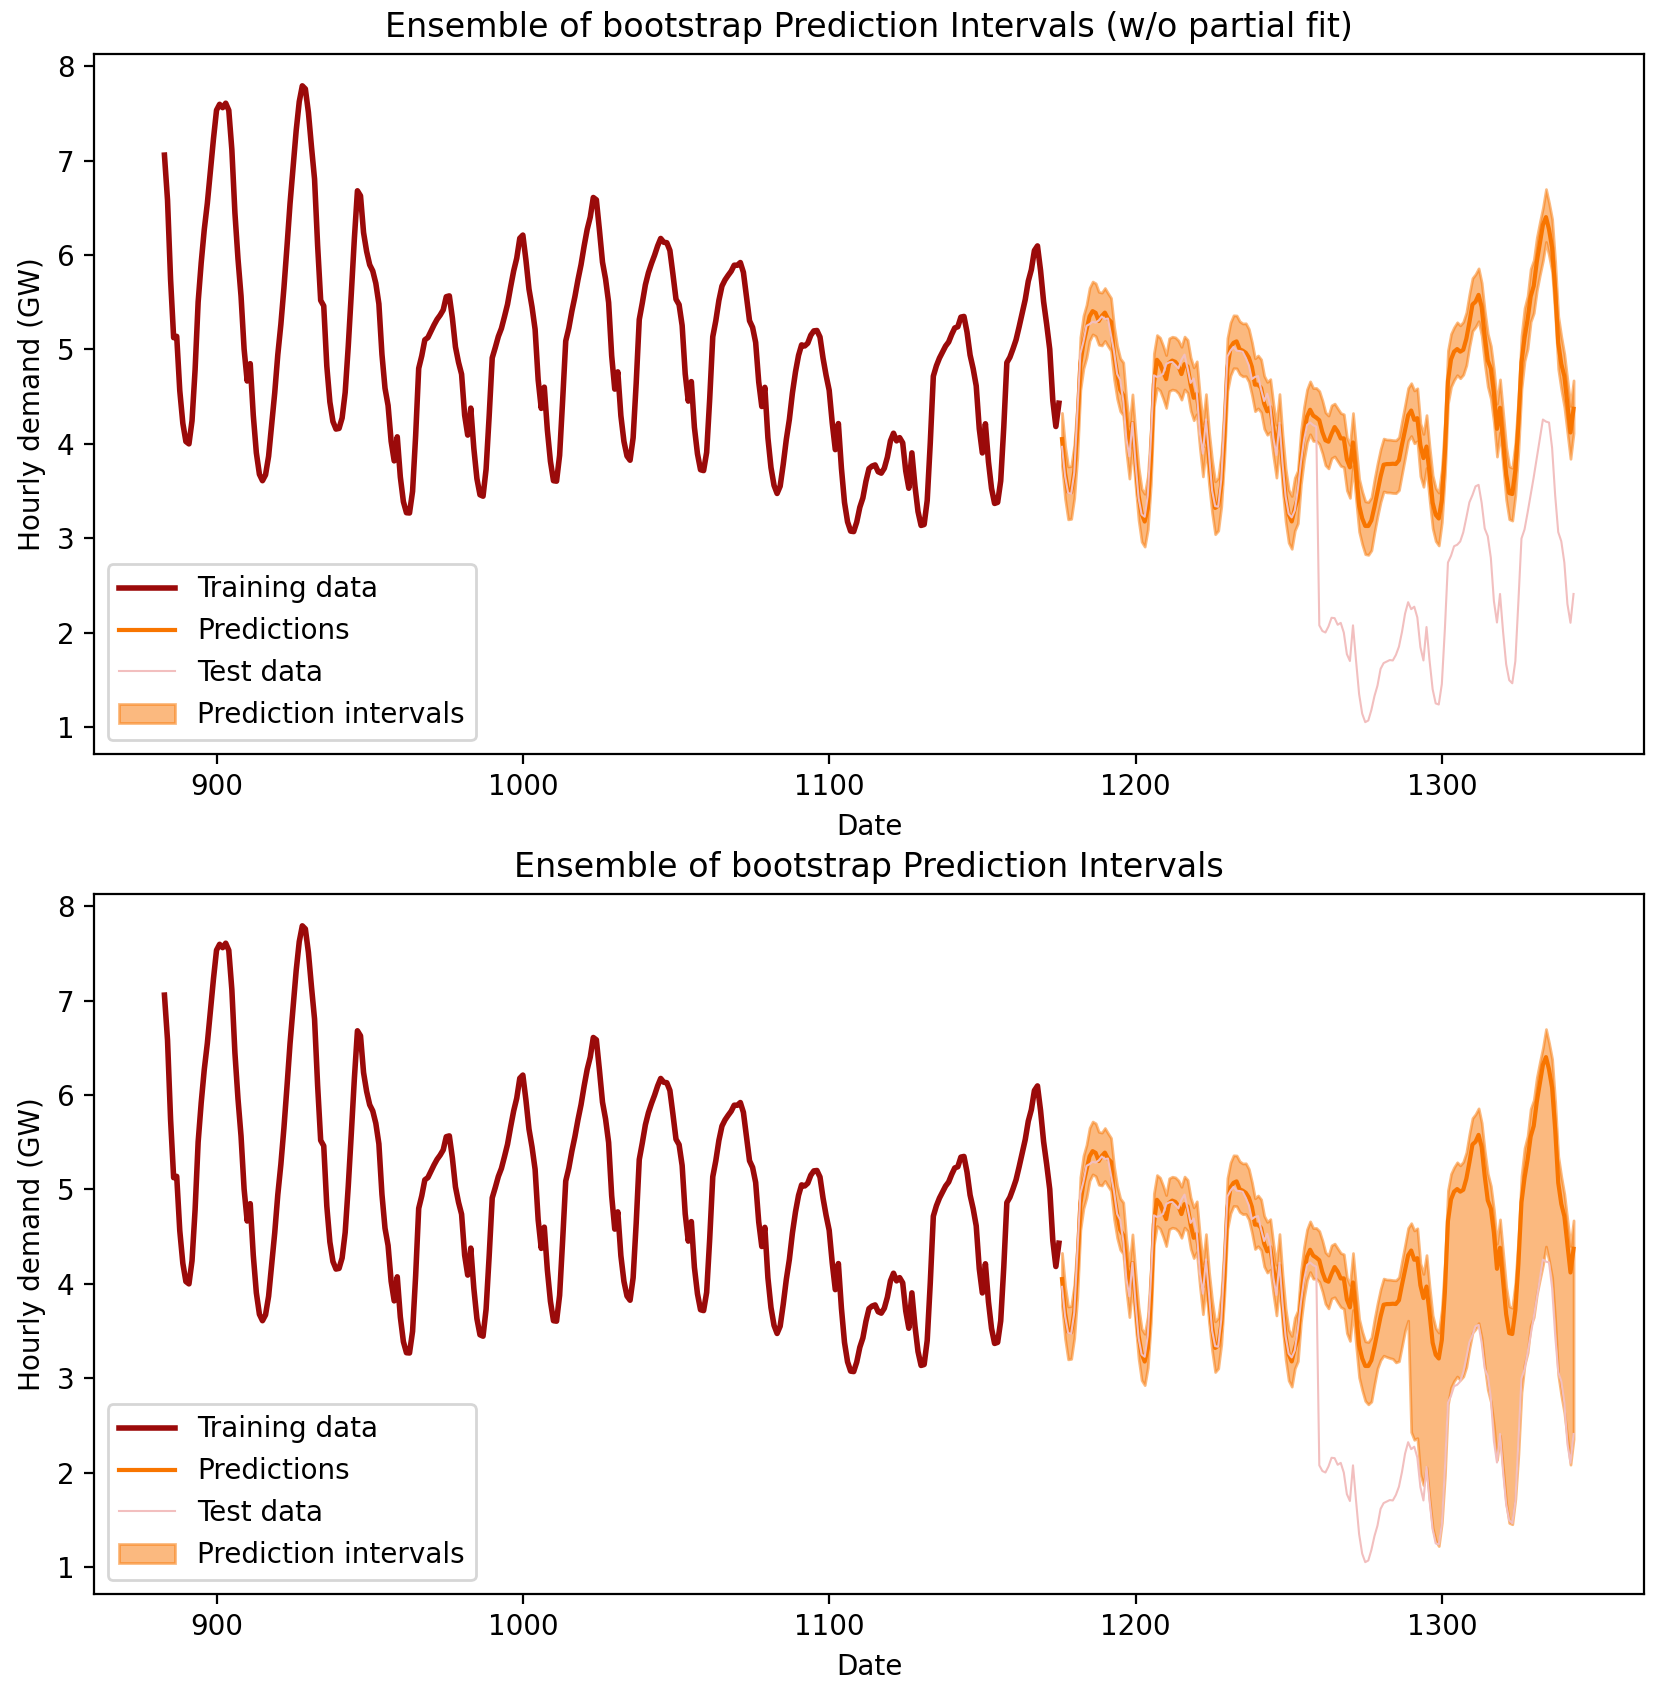
\includegraphics[width=.8\textwidth]{Figures/timeseries/with-change-point/prediction-intervals-timeseries-problem-with-change-point.png}
        \caption{Prediction intervals}
        \label{subfig:app-timeseries-prediction-intervals-cpoint}
    \end{subfigure}
    \hfill % adds horizontal space between figures
    \begin{subfigure}[b]{\textwidth} % Adjust the width to fit your needs
        \centering
        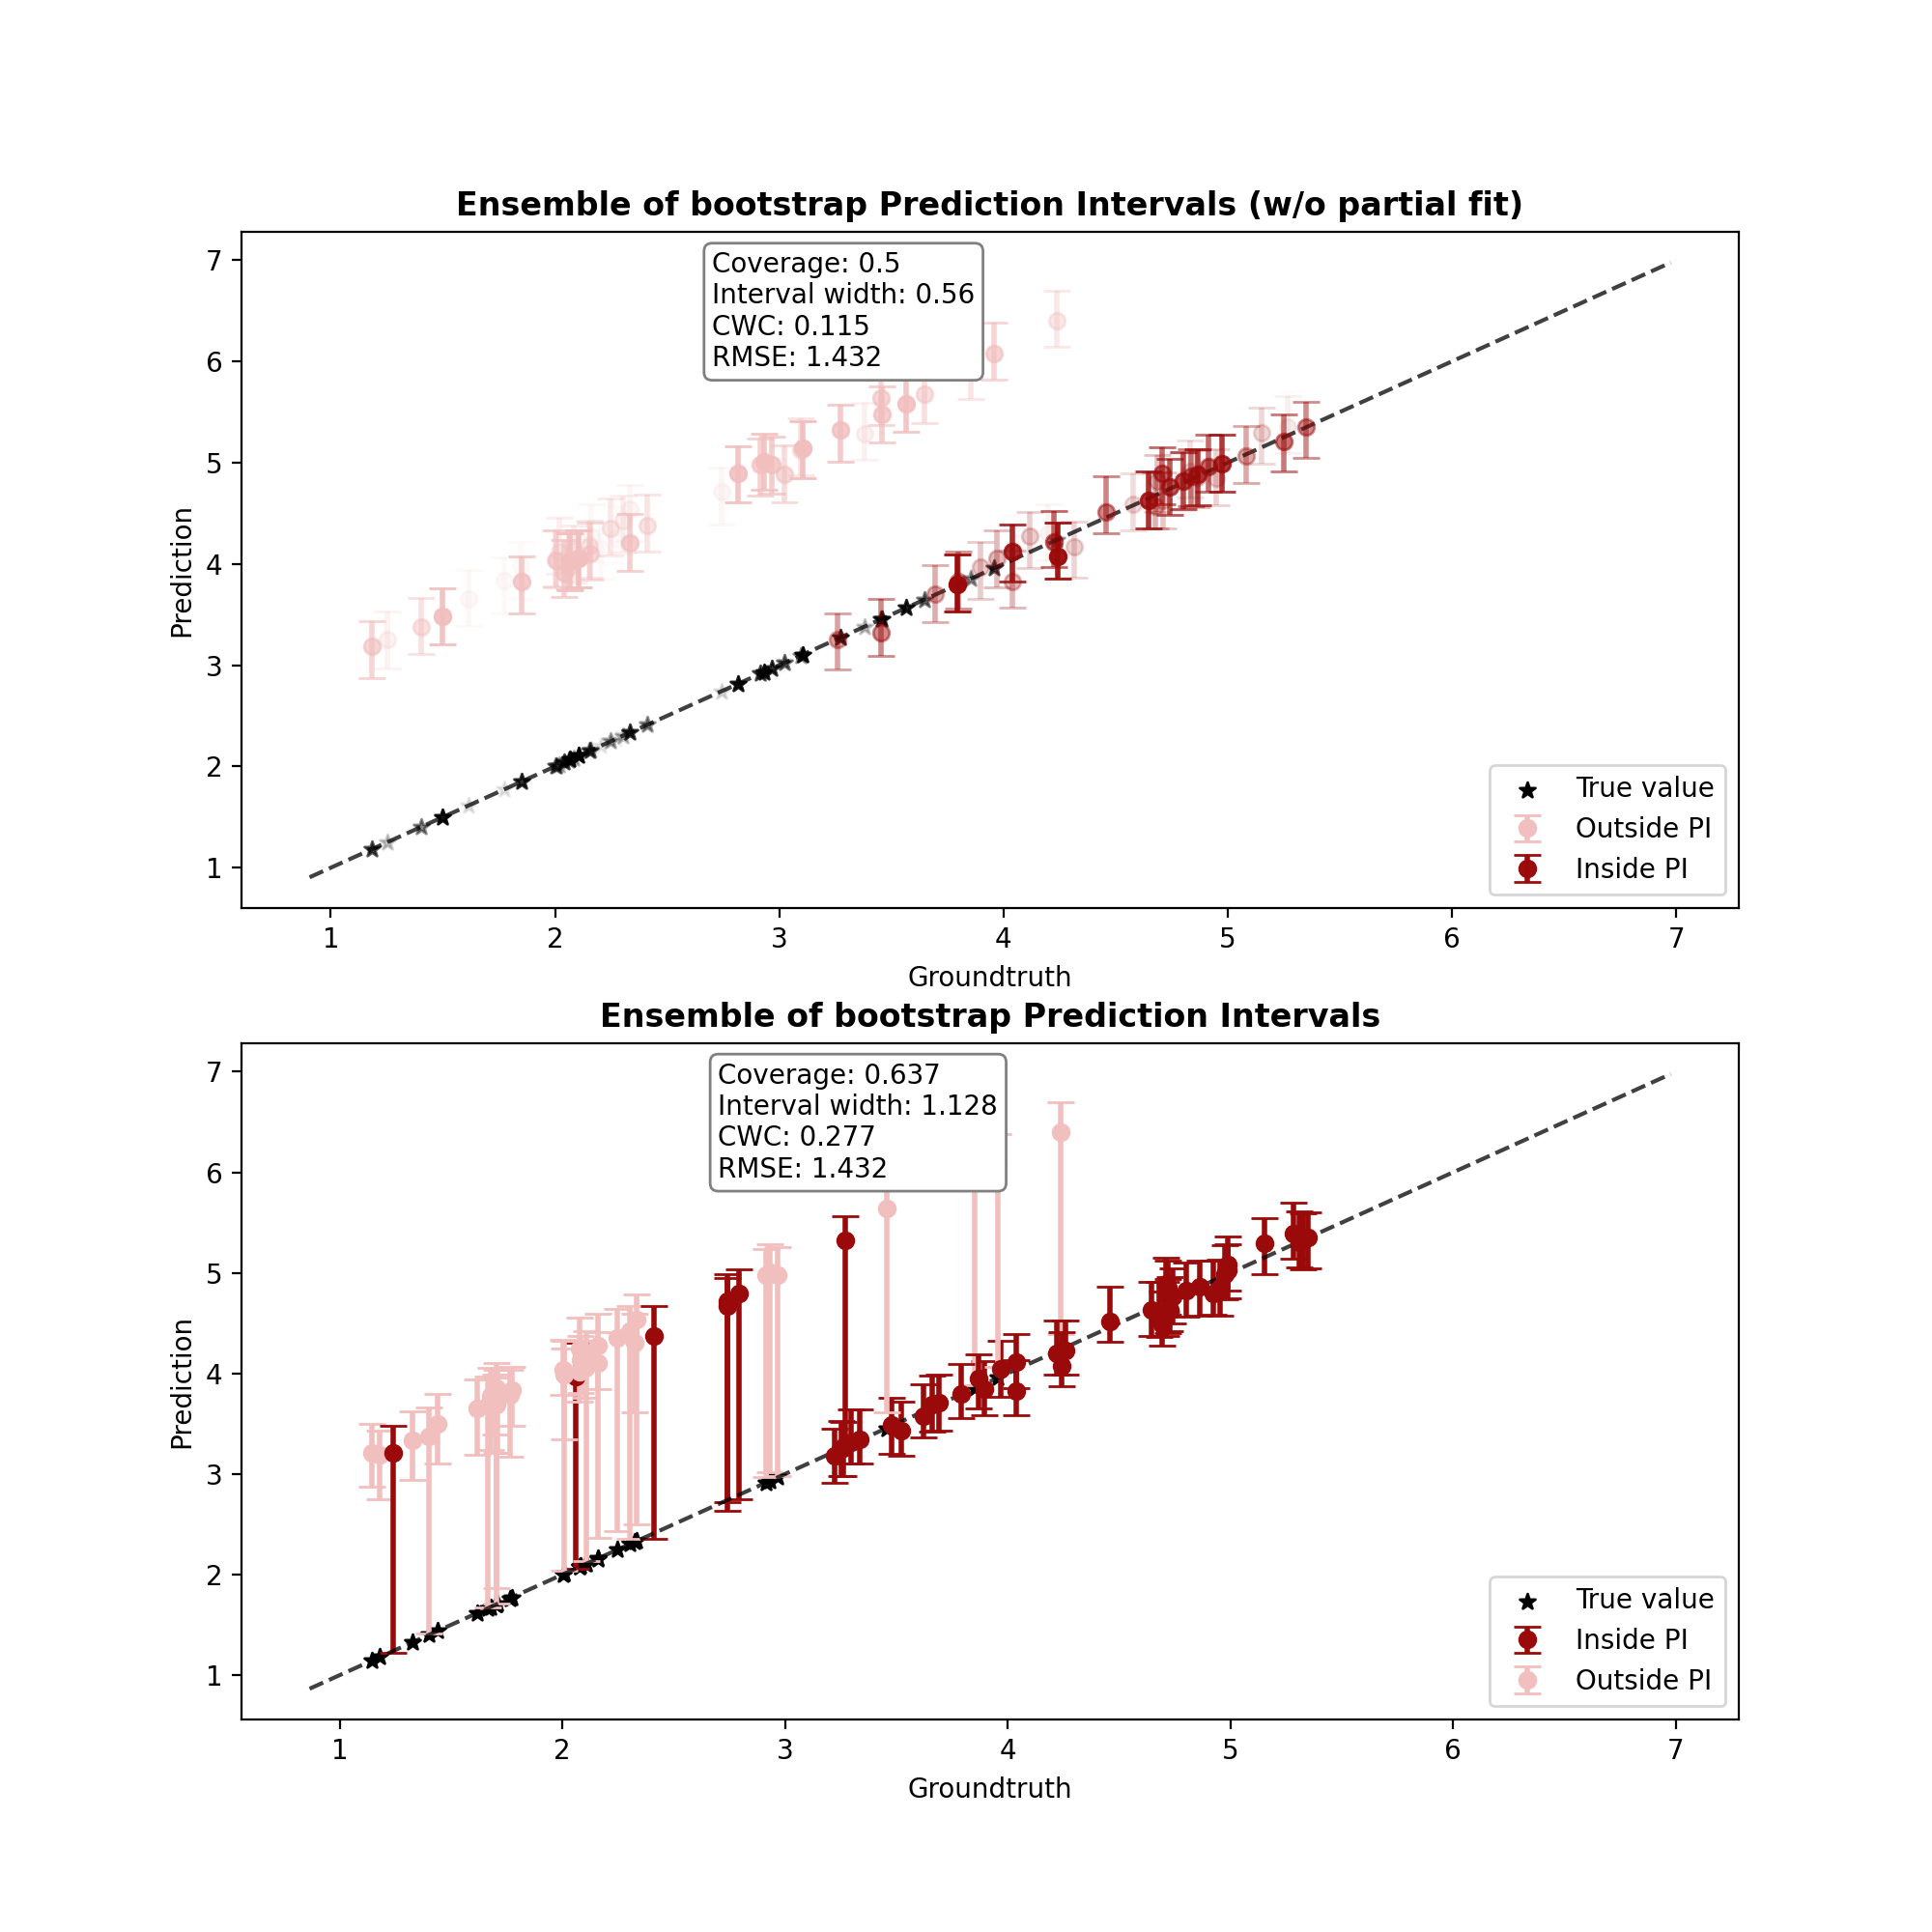
\includegraphics[width=.8\textwidth]{Figures/timeseries/with-change-point/average-goodness-timeseries-problem-with-change-point.png} % Adjust the filename and path
        \caption{Goodness of the prediction intervals (prediction vs. ground truth). Just a $50\%$ of the data is shown due to visualization reasons.}
        \label{subfig:app-timeseries-intervals-goodness-cpoint}
    \end{subfigure}
    \caption{Visualizations related to the prediction intervals for the test data (with a change point) \& the EnbPI strategy (without partial fit, top; and with it, bottom).}
    \label{fig:app-timeseries-intervals-cpoint}
\end{figure}

\begin{figure}[ht]
    \centering
    %\hspace{-10mm}
    \begin{subfigure}[b]{0.32\textwidth}
        \centering
        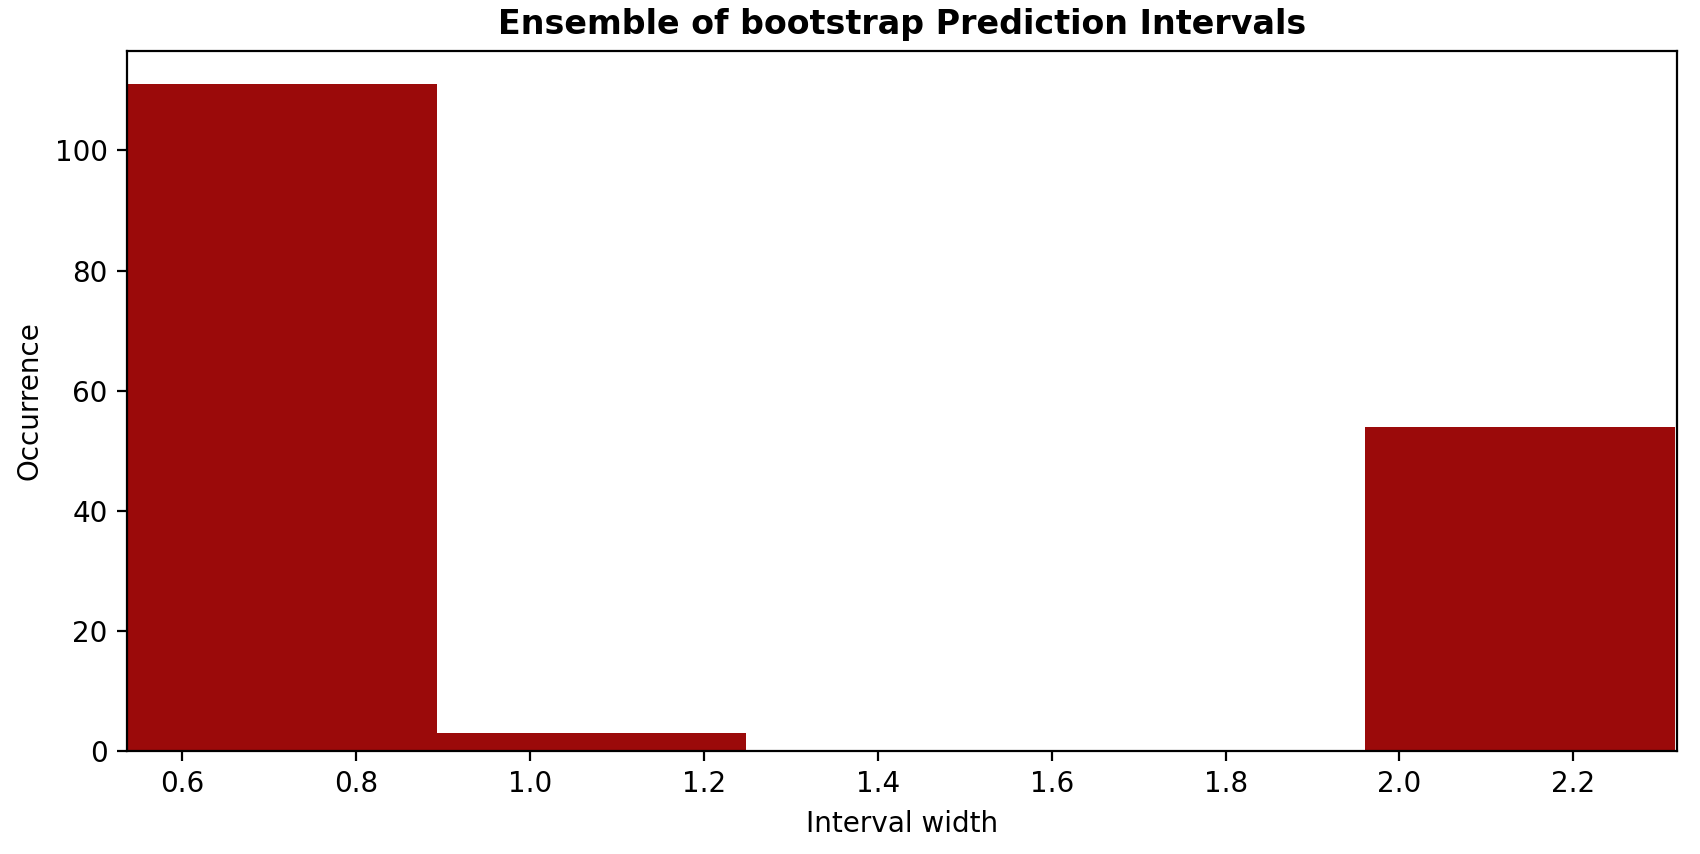
\includegraphics[width=1.15\textwidth, height=1.75\textwidth]{Figures/timeseries/with-change-point/width-occurrence-timeseries-problem-with-change-point.png}
        \caption{Intervals' width histograms}
        \label{subfig:app-timeseries-width-histograms-cpoint}
    \end{subfigure}
    \hfill
    \begin{subfigure}[b]{0.32\textwidth}
        \centering
        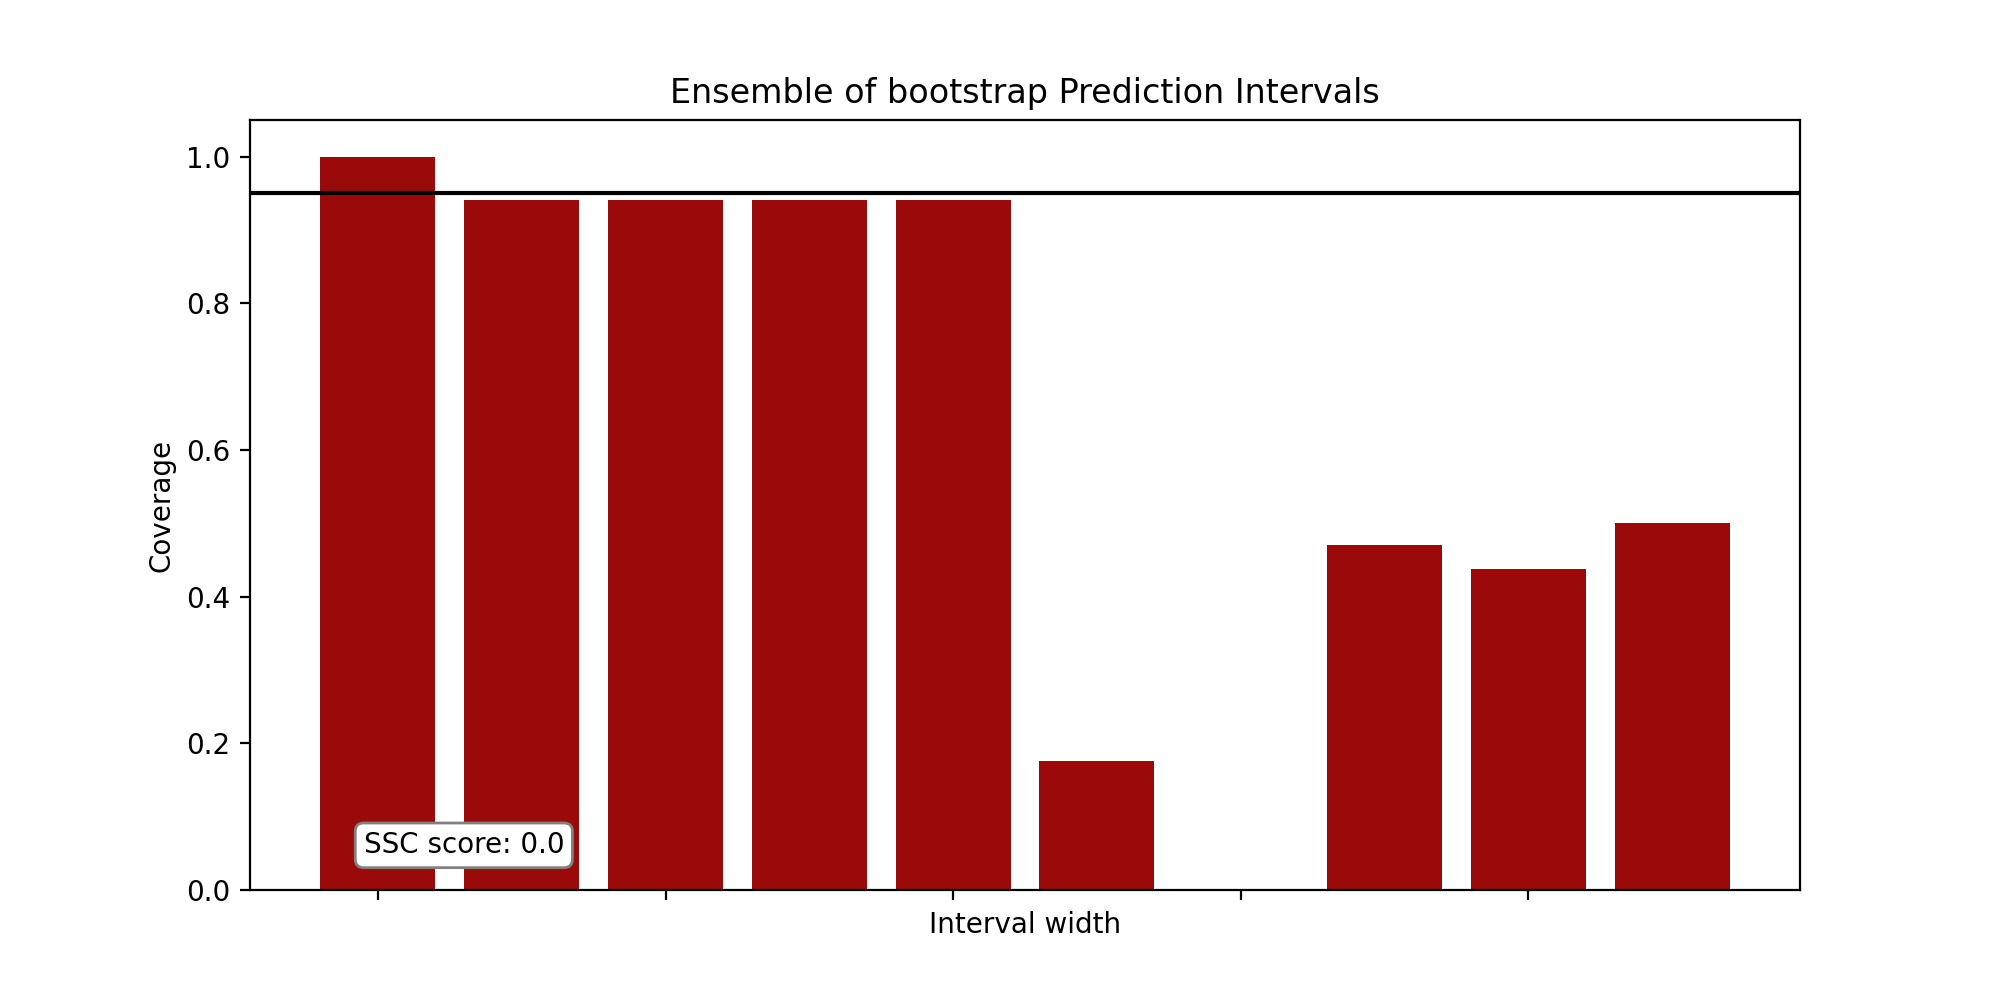
\includegraphics[width=1.15\textwidth, height=0.85\textwidth]{Figures/timeseries/with-change-point/coverage-vs-width-timeseries-problem-with-change-point.png}
        \caption{Coverage in function of intervals' width}
        \label{subfig:app-timeseries-coverage-width-cpoint}
    \end{subfigure}
    \hfill % adds horizontal space between figures
    \begin{subfigure}[b]{0.32\textwidth} % Adjust the width to fit your needs
        \centering
        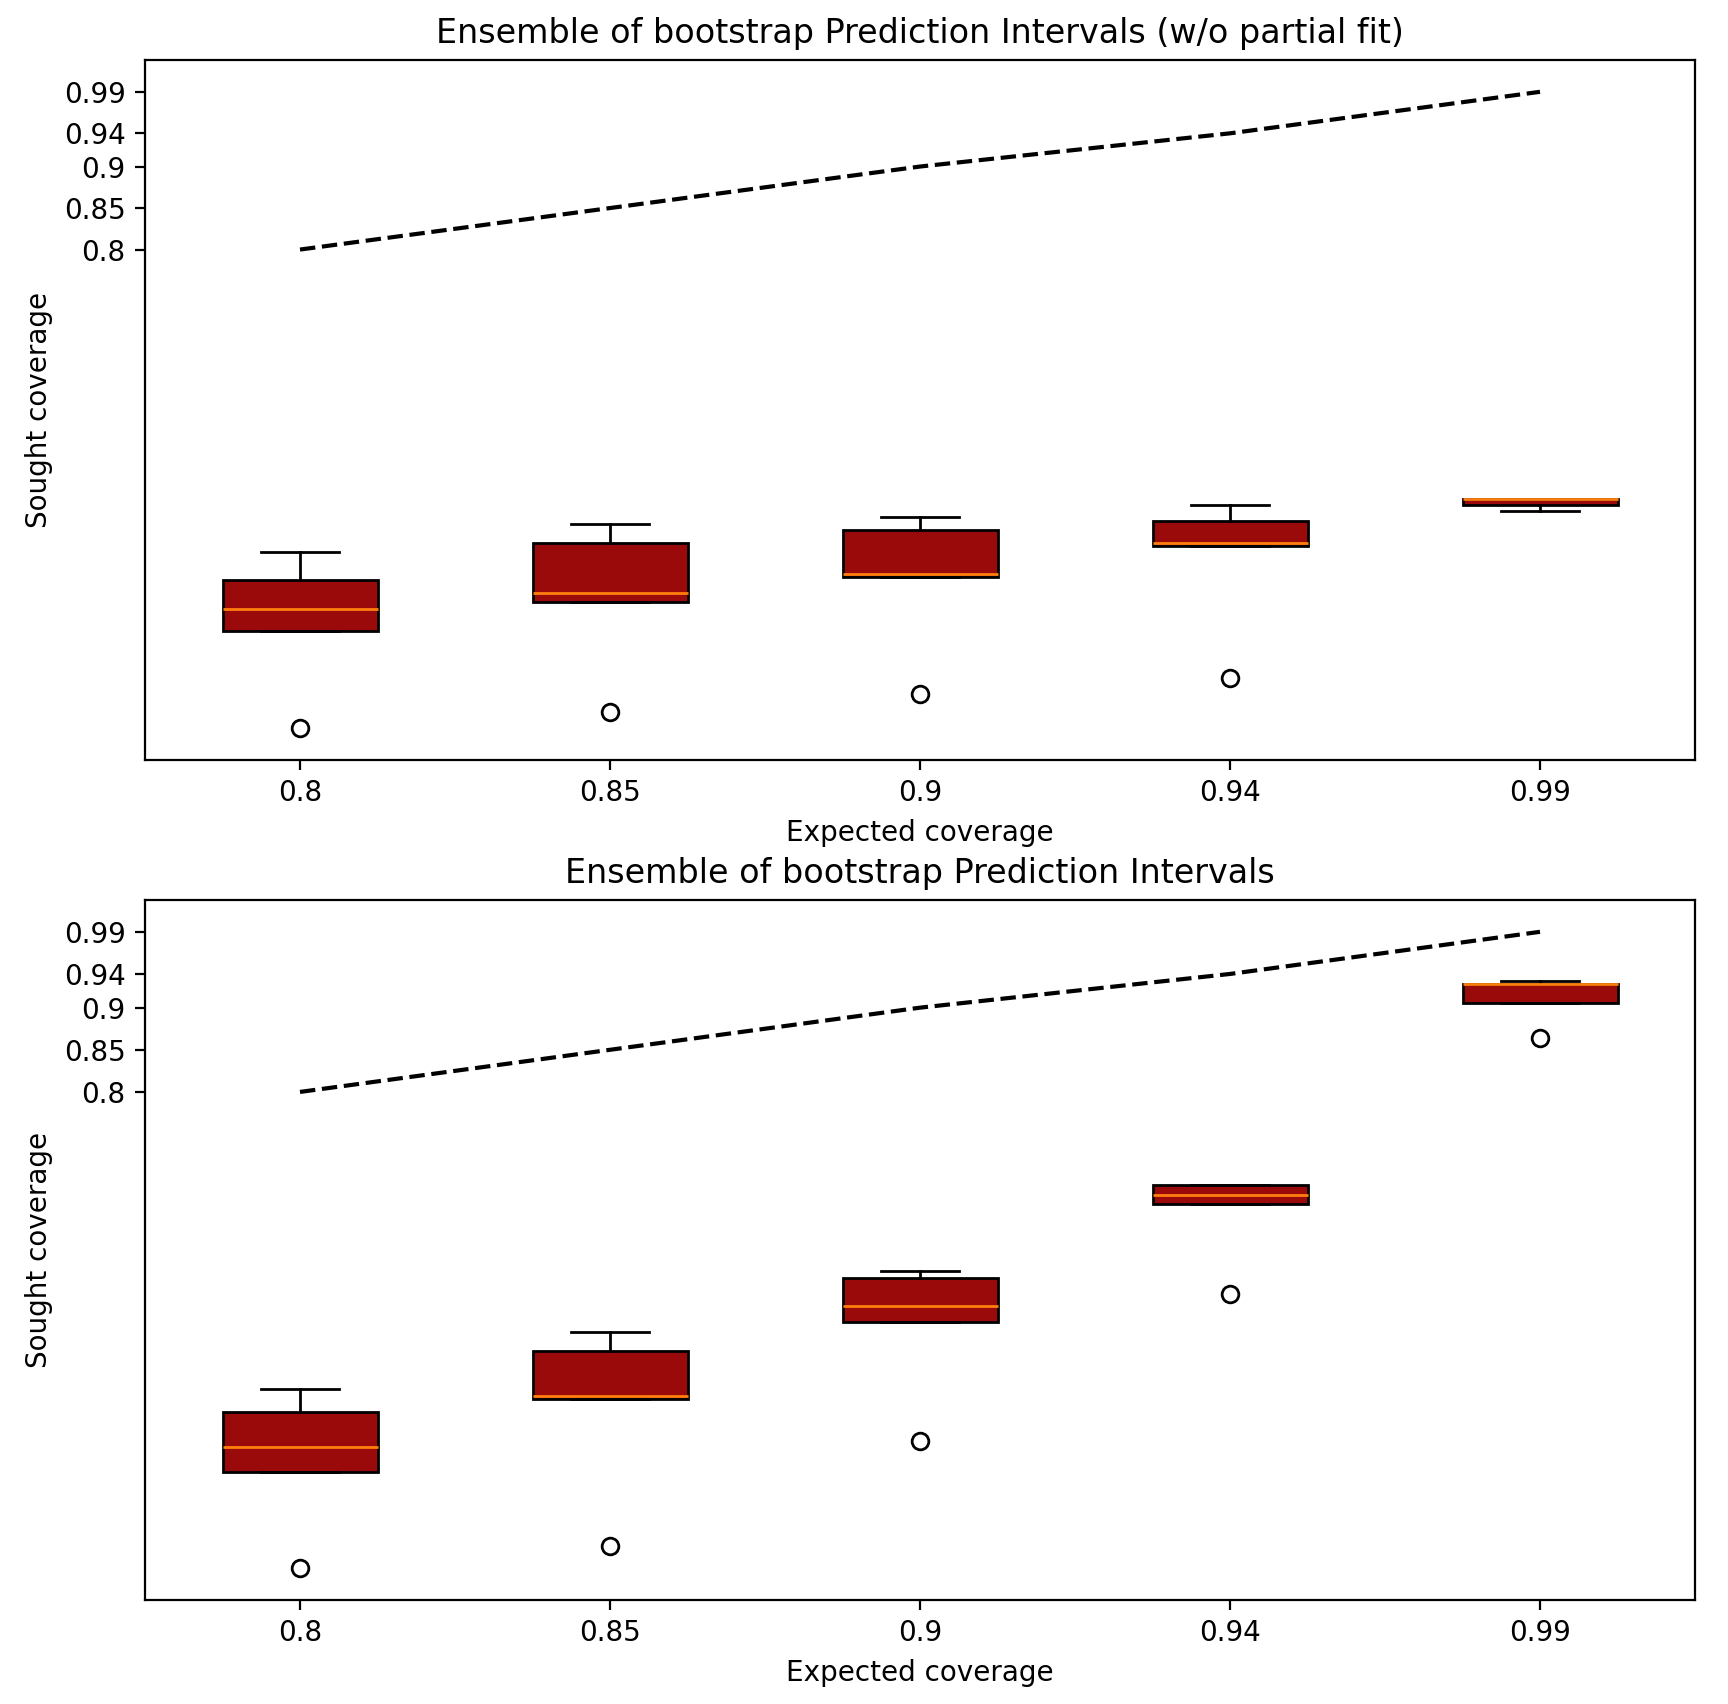
\includegraphics[width=1.15\textwidth, height=1.75\textwidth]{Figures/timeseries/with-change-point/coverage-vs-alpha-timeseries-problem-with-change-problem.png} % Adjust the filename and path
        \caption{Coverage in function of $\a$}
        \label{subfig:app-timeseries-coverage-alpha-cpoint}
    \end{subfigure}
    \caption{Visualizations related to width \& coverage distributions for the test data (with a change point) \& the EnbPI strategy (without partial fit, top; and with it, bottom).}
    \label{fig:app-timeseries-width-coverage-cpoint}
\end{figure}

\begin{figure}[ht]
    \centering
    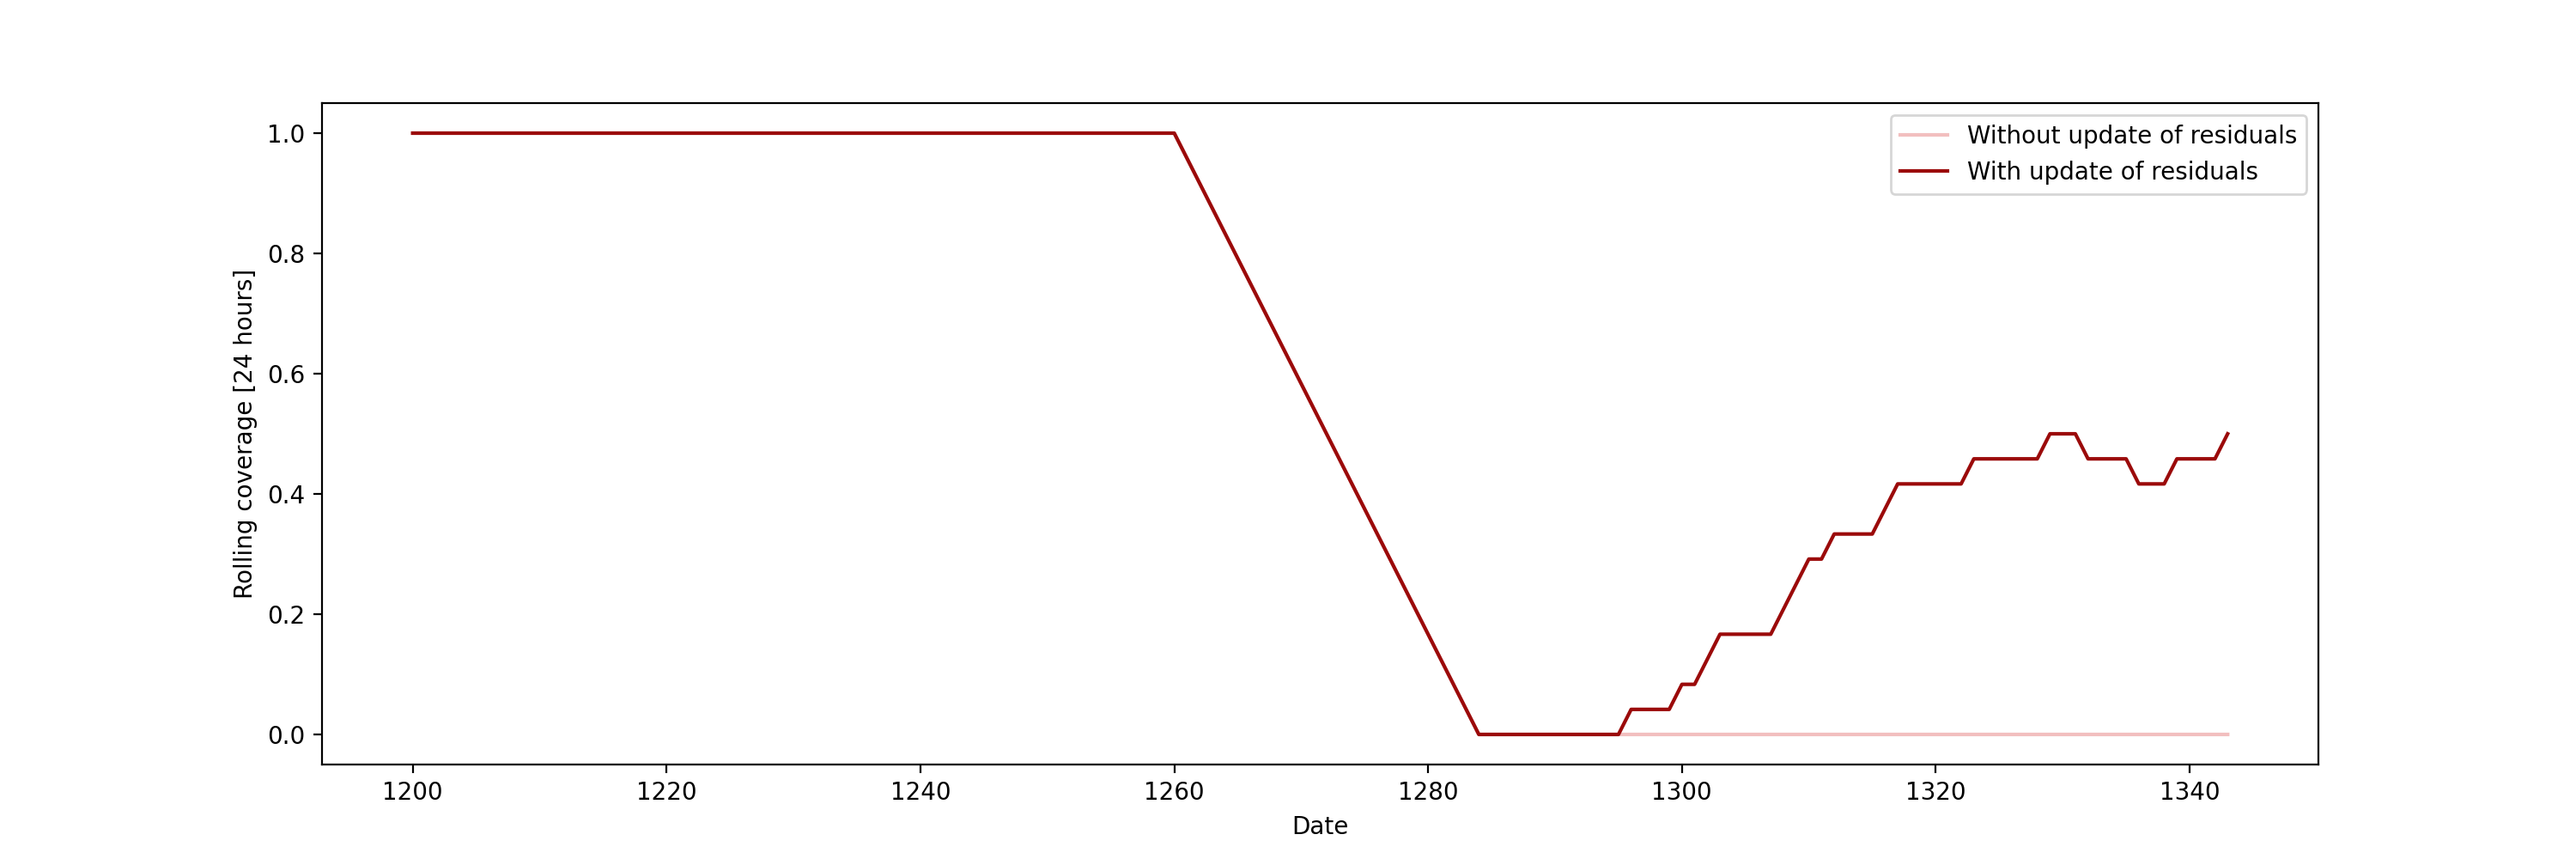
\includegraphics[width=\textwidth]{Figures/timeseries/with-change-point/rolling-coverage-with-change-point.png}
    \caption{Test data coverage (change point's dataset), for the EnbPI strategies, in function of time (grouped within 24h rolling windows).}
    \label{fig:app-timeseries-rolling-coverage-cpoint}
\end{figure}

\begin{figure}[ht]
    \centering
    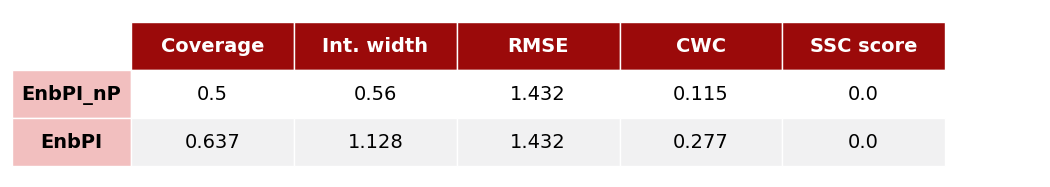
\includegraphics[width=\textwidth]{Figures/timeseries/with-change-point/metrics-table-timeseries-problem-with-change-point.png}
    \caption{Test data metrics for the EnbPI strategy and 1 particular experiment (no 5-folds CV) for $\a=0.05$ and the chage point dataset. From top to bottom: EnbPI without partial fit (EnbPI\_{}nP), EnbPI with it (EnbPI).}
    \label{fig:app-timeseries-metrics-cpoint}
\end{figure}

\begin{figure}[ht]
    \centering
    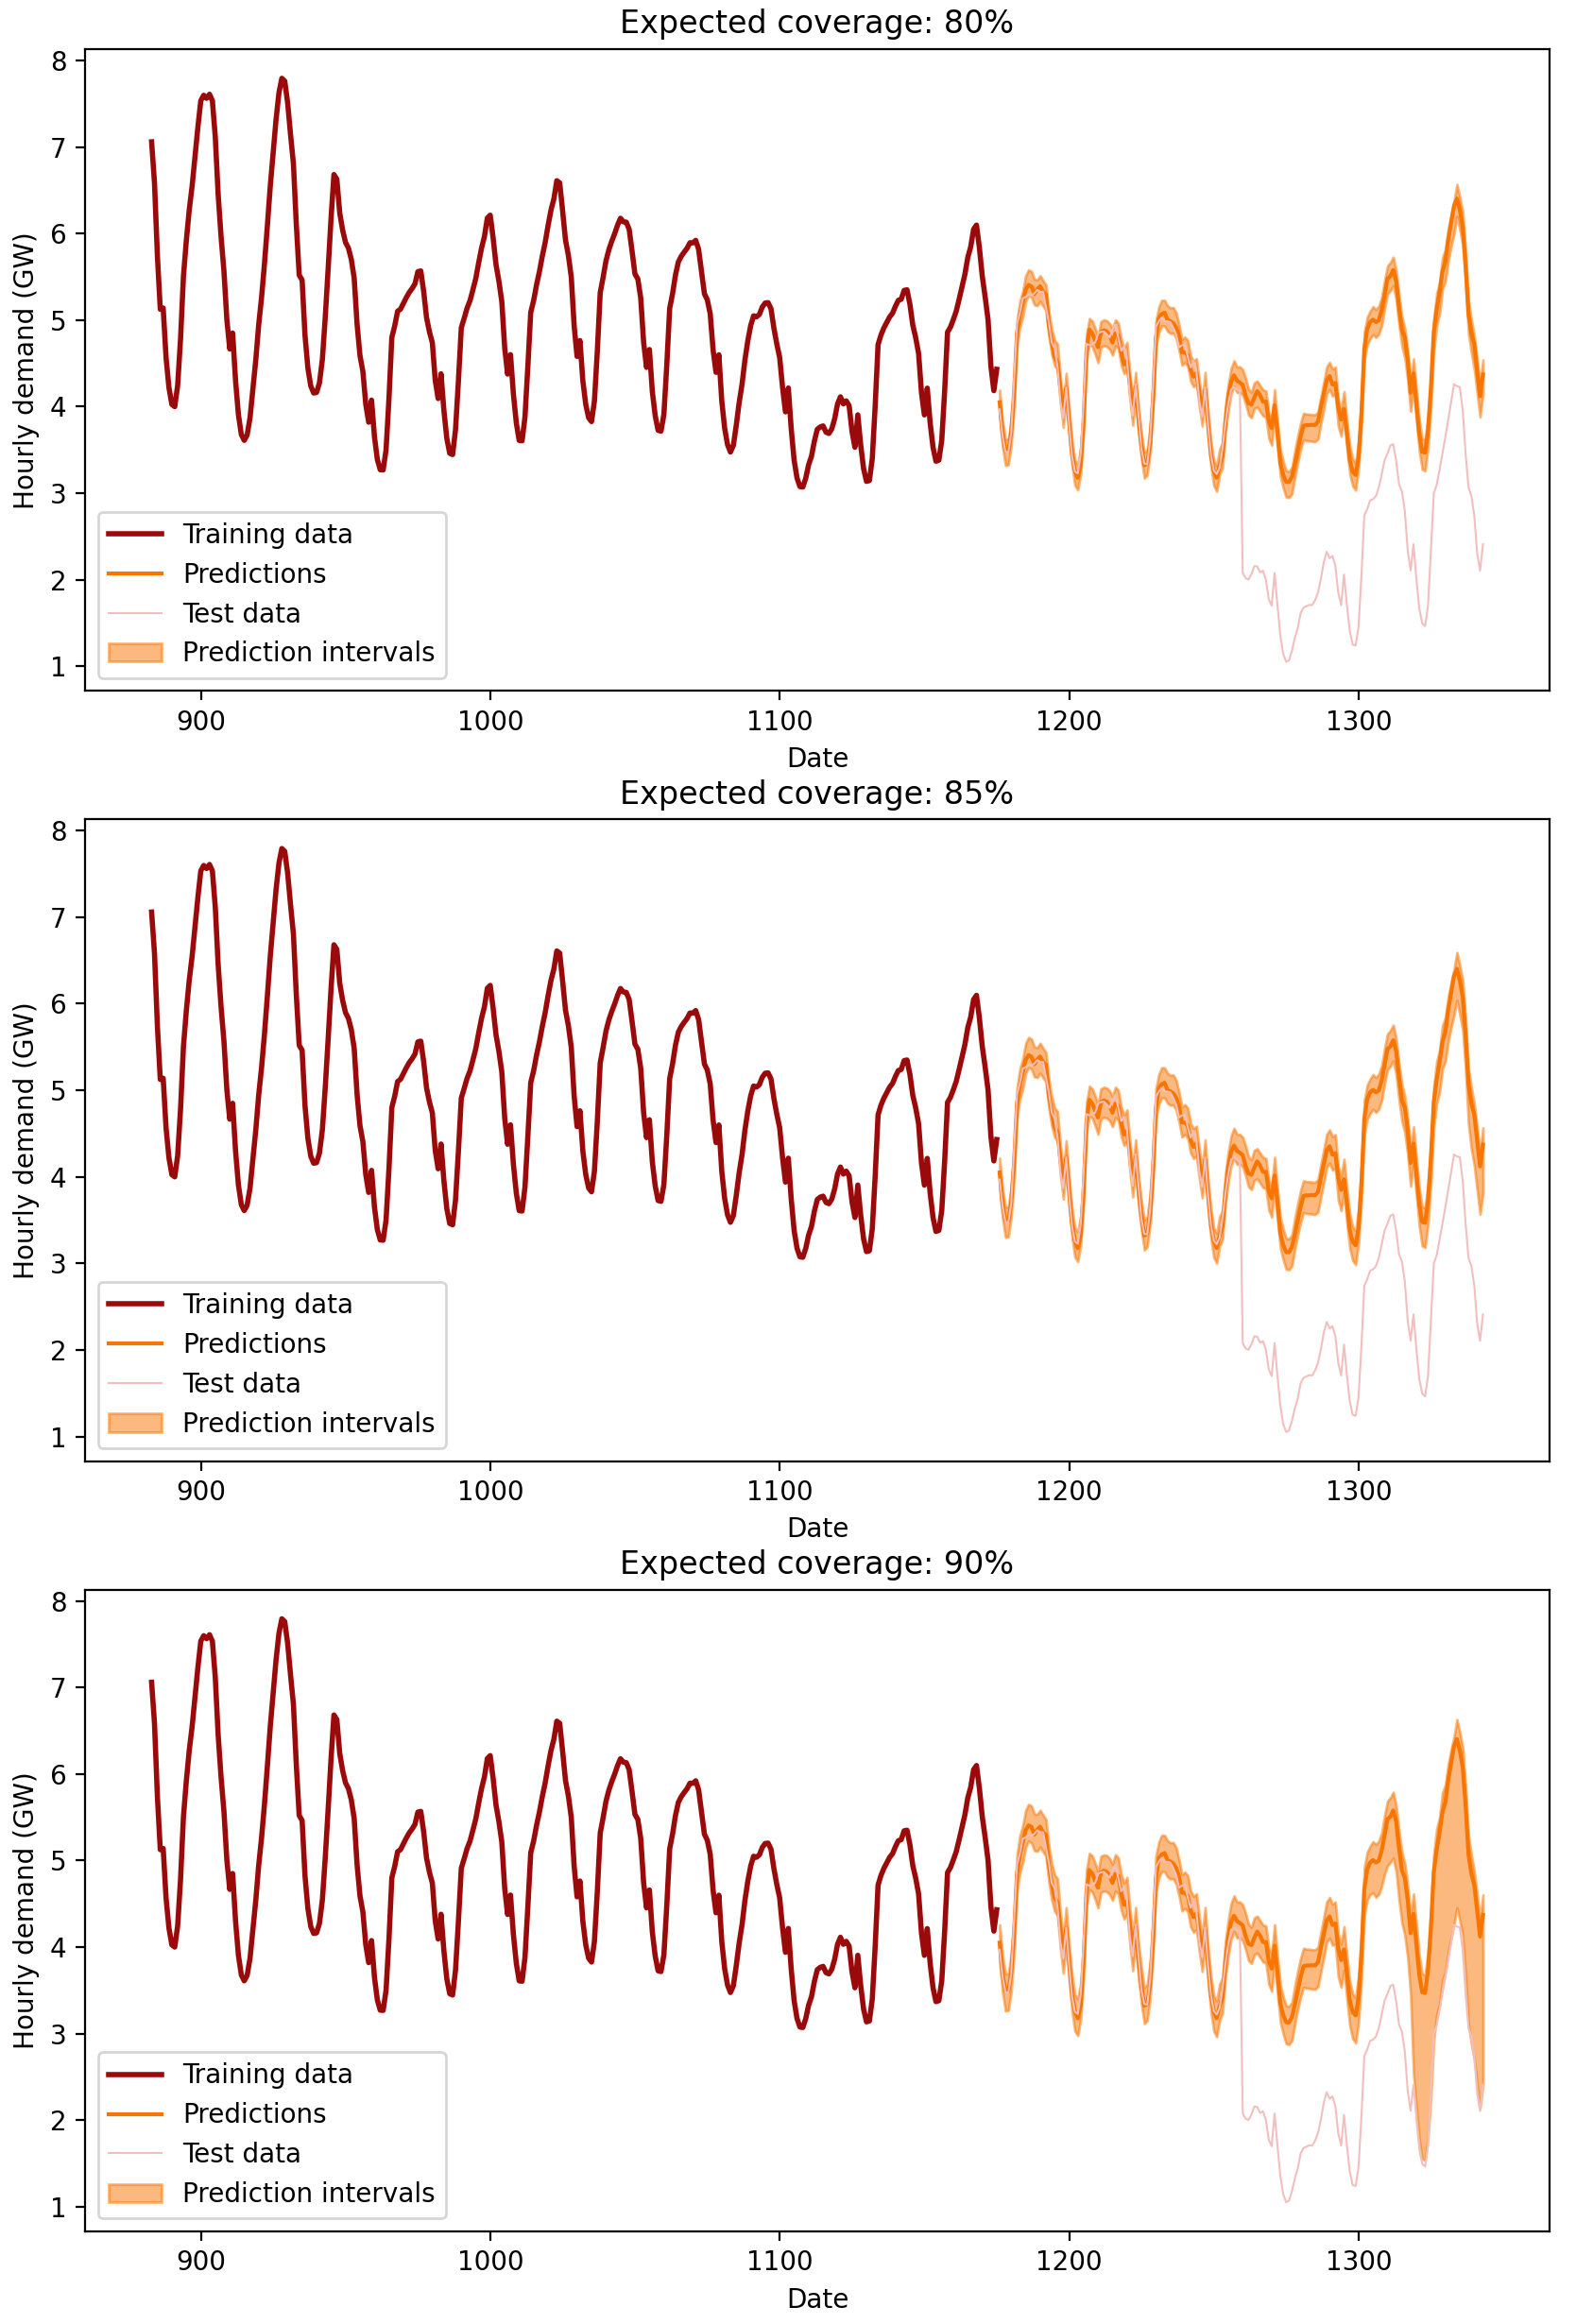
\includegraphics[width=\textwidth]{Figures/timeseries/with-change-point/prediction-intervals-in-function-of-miscoverage.png}
    \caption{Prediction intervals (change point's dataset) in function of time and for different values of $\a$.}
    \label{fig:app-timeseries-intervals-alpha-cpoint}
\end{figure}